%package list
\documentclass{article}
\usepackage[top=3cm, bottom=3cm, outer=3cm, inner=3cm]{geometry}
\usepackage{multicol}
\usepackage{graphicx}
\usepackage{url}
%\usepackage{cite}
\usepackage{hyperref}
\usepackage{array}
%\usepackage{multicol}
\newcolumntype{x}[1]{>{\centering\arraybackslash\hspace{0pt}}p{#1}}
\usepackage{natbib}
\usepackage{pdfpages}
\usepackage{multirow}
\usepackage[normalem]{ulem}
\useunder{\uline}{\ul}{}
\usepackage{svg}
\usepackage{xcolor}
\usepackage{listings}
\lstdefinestyle{ascii-tree}{
    literate={├}{|}1 {─}{--}1 {└}{+}1 
  }
\lstset{basicstyle=\ttfamily,
  showstringspaces=false,
  commentstyle=\color{red},
  keywordstyle=\color{blue}
}
%\usepackage{booktabs}
\usepackage{caption}
\usepackage{subcaption}
\usepackage{float}
\usepackage{array}

\newcolumntype{M}[1]{>{\centering\arraybackslash}m{#1}}
\newcolumntype{N}{@{}m{0pt}@{}}


%%%%%%%%%%%%%%%%%%%%%%%%%%%%%%%%%%%%%%%%%%%%%%%%%%%%%%%%%%%%%%%%%%%%%%%%%%%%
%%%%%%%%%%%%%%%%%%%%%%%%%%%%%%%%%%%%%%%%%%%%%%%%%%%%%%%%%%%%%%%%%%%%%%%%%%%%
\newcommand{\itemEmail}{vmamanian@unsa.edu.pe}
\newcommand{\itemStudent}{Victor Mamani Anahua}
\newcommand{\itemCourse}{Fundamentos de la Programación II}
\newcommand{\itemCourseCode}{20230489}
\newcommand{\itemSemester}{II}
\newcommand{\itemUniversity}{Universidad Nacional de San Agustín de Arequipa}
\newcommand{\itemFaculty}{Facultad de Ingeniería de Producción y Servicios}
\newcommand{\itemDepartment}{Departamento Académico de Ingeniería de Sistemas e Informática}
\newcommand{\itemSchool}{Escuela Profesional de Ingeniería de Sistemas}
\newcommand{\itemAcademic}{2023 - B}
\newcommand{\itemInput}{Del 25 Octubre 2023}
\newcommand{\itemOutput}{Al 1 Noviembre 2023}
\newcommand{\itemPracticeNumber}{10}
\newcommand{\itemTheme}{Laboratorio 10}
%%%%%%%%%%%%%%%%%%%%%%%%%%%%%%%%%%%%%%%%%%%%%%%%%%%%%%%%%%%%%%%%%%%%%%%%%%%%
%%%%%%%%%%%%%%%%%%%%%%%%%%%%%%%%%%%%%%%%%%%%%%%%%%%%%%%%%%%%%%%%%%%%%%%%%%%%

\usepackage[english,spanish]{babel}
\usepackage[utf8]{inputenc}
\AtBeginDocument{\selectlanguage{spanish}}
\renewcommand{\figurename}{Figura}
\renewcommand{\refname}{Referencias}
\renewcommand{\tablename}{Tabla} %esto no funciona cuando se usa babel
\AtBeginDocument{%
	\renewcommand\tablename{Tabla}
}

\usepackage{fancyhdr}
\pagestyle{fancy}
\fancyhf{}
\setlength{\headheight}{30pt}
\renewcommand{\headrulewidth}{1pt}
\renewcommand{\footrulewidth}{1pt}
\fancyhead[L]{\raisebox{-0.2\height}{
\includegraphics[width=3cm]{img/logo_episunsa.png}}}
\fancyhead[C]{\fontsize{7}{7}\selectfont	\itemUniversity \\ \itemFaculty \\ \itemDepartment \\ \itemSchool \\ \textbf{\itemCourse}}
\fancyhead[R]{\raisebox{-0.2\height}{
\includegraphics[width=1.2cm]{img/logo_abet}}}
\fancyfoot[L]{Estudiante Victor Mamani A.}
\fancyfoot[C]{\itemCourse}
\fancyfoot[R]{Página \thepage}

% para el codigo fuente
\usepackage{listings}
\usepackage{color, colortbl}
\definecolor{dkgreen}{rgb}{0,0.6,0}
\definecolor{gray}{rgb}{0.5,0.5,0.5}
\definecolor{mauve}{rgb}{0.58,0,0.82}
\definecolor{codebackground}{rgb}{0.95, 0.95, 0.92}
\definecolor{tablebackground}{rgb}{0.8, 0, 0}

\lstdefinestyle{java}{frame=tb,
	language=Java,
	showstringspaces=false,
	columns=flexible,
	basicstyle={\footnotesize\ttfamily\color[RGB]{255,255,255}},
	numberstyle=\color{mygray},
	numbers=left, 
	keywordstyle=\color{myblue},
	morekeywords={String, System},
	commentstyle=\color{mygray},
	stringstyle=\color{mygreen},
	breaklines=true,
	breakatwhitespace=true,
	tabsize=2,
	backgroundcolor= \color{codebackgroundCode},
	showspaces=false,
	showtabs=false,
	showlines=false,
}

\lstset{frame=tb,
	language=bash,
	aboveskip=3mm,
	belowskip=3mm,
	showstringspaces=false,
	columns=flexible,
	basicstyle={\small\ttfamily},
	numbers=none,
	numberstyle=\tiny\color{gray},
	keywordstyle=\color{blue},
	commentstyle=\color{dkgreen},
	stringstyle=\color{mauve},
	breaklines=true,
	breakatwhitespace=true,
	tabsize=3,
	backgroundcolor= \color{codebackground},
}

\begin{document}
	
	\vspace*{10px}
	
	\begin{center}	
		\fontsize{17}{17} \textbf{ Informe de Laboratorio \itemPracticeNumber}
	\end{center}
	\centerline{\textbf{\Large Tema: \itemTheme}}
	%\vspace*{0.5cm}	

	\begin{flushright}
		\begin{tabular}{|M{2.5cm}|N|}
			\hline 
			\rowcolor{tablebackground}
			\color{white} \textbf{Nota}  \\
			\hline 
			     \\[30pt]
			\hline 			
		\end{tabular}
	\end{flushright}	

	\begin{table}[H]
		\begin{tabular}{|x{4.7cm}|x{4.8cm}|x{4.8cm}|}
			\hline 
			\rowcolor{tablebackground}
			\color{white} \textbf{Estudiante} & \color{white}\textbf{Escuela}  & \color{white}\textbf{Asignatura}   \\
			\hline 
			{\itemStudent \par \itemEmail} & \itemSchool & {\itemCourse \par Semestre: \itemSemester \par Código: \itemCourseCode}     \\
			\hline 			
		\end{tabular}
	\end{table}		
	
	\begin{table}[H]
		\begin{tabular}{|x{4.7cm}|x{4.8cm}|x{4.8cm}|}
			\hline 
			\rowcolor{tablebackground}
			\color{white}\textbf{Laboratorio} & \color{white}\textbf{Tema}  & \color{white}\textbf{Duración}   \\
			\hline 
			\itemPracticeNumber & \itemTheme & 04 horas   \\
			\hline 
		\end{tabular}
	\end{table}
	
	\begin{table}[H]
		\begin{tabular}{|x{4.7cm}|x{4.8cm}|x{4.8cm}|}
			\hline 
			\rowcolor{tablebackground}
			\color{white}\textbf{Semestre académico} & \color{white}\textbf{Fecha de inicio}  & \color{white}\textbf{Fecha de entrega}   \\
			\hline 
			\itemAcademic & \itemInput &  \itemOutput  \\
			\hline 
		\end{tabular}
	\end{table}
	
	\section{Tarea}
	\begin{itemize}		
        \item Cree un Proyecto llamado Laboratorio10
        \item Crear 3 constructores sobrecargados.
        \item La actitud puede ser defensiva, ofensiva, fuga. Dicha actitud varía cuando el soldado defiende, ataca o huye respectivamente.
        \item Al atacar el soldado avanza, al avanzar aumenta su velocidad en 1. Al defender el soldado se para. Al huir aumenta su velocidad en 2. Al retroceder, si su velocidad es mayor que 0, entonces primero para y su actitud es defensiva, y si su velocidad es 0 entonces disminuirá a valores negativos. Al ser atacado su vida actual disminuye y puede llegar incluso a morir.
        \item Crear los atributos y métodos extra que considere necesarios.
		\item Usted deberá crear las dos clases Soldado.java y VideoJuego5.java. Puede reutilizar lo desarrollado en Laboratorios anteriores.
		\item Del Soldado nos importa el nombre, puntos de vida, fila y columna (posición en el tablero).
		\item El juego se desarrollará en el mismo tablero de los laboratorios anteriores. Para el tablero utilizar la estructura de datos más adecuada.
		\item Tendrá 2 Ejércitos. Inicializar el tablero con n soldados aleatorios entre 1 y 10 para cada Ejército. Cada soldado tendrá un nombre autogenerado: Soldado0X1, Soldado1X1, etc., un valor de puntos de vida autogenerado aleatoriamente [1..5], la fila y columna también autogenerados aleatoriamente (no puede haber 2 soldados en el mismo cuadrado). 
		\item Además de los datos del Soldado con mayor vida de cada ejército, el promedio de puntos de vida de todos los soldados creados por ejército, los datos de todos los soldados porejército en el orden que fueron creados y un ranking de poder de todos los soldados creados por ejército (del que tiene más nivel de vida al que tiene menos) usando 2 diferentes algoritmos de ordenamiento (indicar conclusiones respecto a este ordenamiento de HashMaps).
		\item Finalmente, que muestre qué ejército ganará la batalla (indicar la métrica usada para decidir al ganador de la batalla).
		\item Crear el diagrama de clases UML.
		\item El juego es humano contra humano y consistirá en mover un soldado por cada turno de cada jugador. Se puede mover en cualquier dirección, Ud. deberá darle la coordenada del soldado a mover y la dirección de movimiento, el programa deberá verificar que hay un soldado del ejército que corresponda en dicha posición y que el movimiento es válido (no puede haber 2 soldados del mismo ejército en el cuadrado y no se puede ordenar moverse a una posición fuera del tablero), pidiendo ingresar nuevos datos si no es así.
		\item Cuando un soldado se mueve a una posición donde hay un soldado rival, se produce una batalla y gana el soldado que tenga mayor nivel de vida actual. Gana el juego quien deje al otro ejército vacío. Después de cada movida se deberá mostrar el tablero con su estado actual. Hacer un programa iterativo.
	\end{itemize}

	\section{Equipos, materiales y temas utilizados}
	\begin{itemize}
		\item Sistema Operativo Ubuntu GNU Linux 23 lunar 64 bits Kernell 6.2.v
		\item Visual Studio Code.
		\item VIM 9.0.
		\item OpenJDK 64-Bits 19.0.7.
		\item Git 2.39.2.
		\item Cuenta en GitHub con el correo institucional.
		\item Programación Orientada a Objetos.
		\item Actividades del Laboratorio 10.	
	\end{itemize}
	
	\section{URL de Repositorio Github}
	\begin{itemize}
		\item URL del Repositorio GitHub para clonar o recuperar.
		\item \url{https://github.com/VictorMA18/fp2-23b.git}
		\item URL para el laboratorio 10 en el Repositorio GitHub.
		\item \url{https://github.com/VictorMA18/fp2-23b/tree/main/Fase02/Lab10}
	\end{itemize}
	
	\section{Actividades del Laboratorio 10}

	\subsection{Ejercicio Soldado}
	\begin{itemize}	
		\item En el primer commit agregando la clase soldado que esta siendo reutilizada para podef reslizar el siguiente ejercicio.
		\item El codigo y el commit seria el siguiente:
	\end{itemize}	
	\begin{lstlisting}[language=bash,caption={Commit}][H]
		$ git commit -m "Agregando la clase soldado para podef reslizar el siguiente ejercicio "
	\end{lstlisting}	
	\begin{lstlisting}[language=java,caption={Las lineas de codigos del metodo creado:}][H]
		// Laboratorio Nro 10 - Ejercicio Soldado
		// Autor: Mamani Anahua Victor Narciso
		// Colaboro:
		// Tiempo:
		import java.util.*;
		public class Soldado { //CREAMOS LA CLASE SOLDODADO PARA PODER USAR UN ARREGLO BIDIMENSIONAL DONDE NECESITAMOS LA VIDA , EL NOMBRE DEL SOLDADO Y TAMBIEN SU POSICION COMO LA FILA Y LA COLUMNA   
		
			private String name;
			private int lifeactual;
			private int row;
			private String column;
			private int attacklevel;
			private int defenselevel;
			private int lifelevel;
			private int speed;
			private String attitude;
			private boolean lives;
		
			Random rdm = new Random();
		
			//Anadiendo metodo que nos permita que un arreglo tenga datos nulos si este esta vacio
			public Soldado(){
				this.name = "";
				this.row = 0;
				this.column  = "";
				this.attacklevel = 0;
				this.defenselevel = 0;
				this.lifelevel = 0
				this.lifeactual = 0;
				this.speed = 0;
				this.attitude = "";
				this.lives = false;
			}
		
			//Constructor
			public Soldado(String name, int health, int row, String column){
				this.name = name;
				this.lifeactual = health;
				this.lifelevel = health;
				this.lifeactual = health;
				this.row = row;
				this.column = column;
				this.lives = true;
				
				//YA QUE ESTOS DATOS SERIAN ALEATORIOS YA QUE SE ESTARIA CREANDO EL SOLDADO TENDRIAMOS DATOS QUE SERIAN COMO ATTACKLEVEL DEFENSELEVEL EL CUAL TENDRIAN QUE SER ALEATORIOS    
				this.attacklevel = rdm.nextInt(5) + 1;
				this.defenselevel = rdm.nextInt(5) + 1;
		
			}
			
			//Constructor para los diferentes niveles como de vidad defensa ataque velocidad
			public Soldado(String name , int attacklevel, int defenselevel, int lifelevel, int speed, boolean lives, int row, String column) {
				this.name = name;
				this.attacklevel = attacklevel;
				this.defenselevel = defenselevel;
				this.lifelevel = lifelevel;
				this.speed = speed;
				this.lives = lives;
				this.row = row;
				this.column = column;
			}
		
			//Metodos necesarios como avanzar defender huir al seratacado al retroceder
			public void advance(){
				this.speed = getSpeed() + 1;
				System.out.println("El soldado " + this.name + "avanzo");
			}
			public void defense(){
				this.speed = 0;
				this.attitude = "DEFENSIVA";
				System.out.println("El soldado " + this.name + "esta defendiendo");
			}
			public void flee(){
				this.speed = getSpeed() + 2;
				this.attitude = "HUYE";
				System.out.println("El soldado " + this.name + "esta huyendo");
			}
			public void back(){
				System.out.println("El soldado " + this.name + "esta retrocediendo");
				if(this.speed == 0){
					this.speed = rdm.nextInt(5) - 5;
				}else{
					if(this.speed > 0){
						this.speed = 0;
						this.attitude = "DEFENSIVA";
					}
				}
			}
			public void attack(Soldado soldier){
				if(this.getLifeActual() > soldier.getLifeActual()){
					int life = this.getLifeActual() - soldier.getLifeActual();
					this.setLifeActual(life);
					this.setLifeLevel(life);
					soldier.lives = false;
					System.out.println(this.name + " asesino al soldado " + soldier.name);
				}else if(soldier.getLifeActual() > this.getLifeActual()){
					int life = soldier.getLifeActual() - this.getLifeActual();
					this.lives = false;
					soldier.setLifeActual(life);
					soldier.setLifeLevel(life);
					System.out.println(soldier.name + " asesino al soldado " + this.name);
				}else{
					this.lives = false;
					soldier.lives = false;
					System.out.println("los 2 soldados se asesinaron");
				}
			}
			public void morir(){
				this.lives = false;
				this.attitude = "SOLDADO MUERTO";
			}
		
			// Metodos mutadores
			public void setName(String n){
				name = n;
			}
			public void setLifeActual(int p){
				lifeactual = p;
			}
			public void setRow(int b){
				row = b;
			}
			public void setColumn(String c){
				column = c; 
			}
			public void setAttackLevel(int attacklevel) {
				this.attacklevel = attacklevel;
			}
			public void setDefenseLevel(int defenselevel) {
				this.defenselevel = defenselevel;
			}
			public void setLifeLevel(int lifelevel){
				this.lifelevel = lifelevel;
			}
			public void setSpeed(int speed) {
				this.speed = speed;
			}
			public void setAttitude(String attitude) {
				this.attitude = attitude;
			}
			public void setLives(boolean lives) {
				this.lives = lives;
			}
		
			// Metodos accesores
			public String getName(){
				return name;
			}
			public int getLifeActual(){
				return lifeactual;
			}
			public int getRow(){
				return row;
			}
			public String getColumn(){
				return column;
			}
			public int getAttackLevel() {
				return attacklevel;
			}
			public int getDefenseLevel() {
				return defenselevel;
			}
			public int getLifeLevel(){
				return lifelevel;
			}
			public int getSpeed() {
				return speed;
			}
			public String getAttitude() {
				return attitude;
			}
			public boolean getLives() {
				return lives;
			}
		
			// Completar con otros metodos necesarios
			public String toString(){ //CREAMOS ESTE METODO PARA IMPRIMIR LOS DATOS DEl OBJETO
				String join = "\nNombre: " + getName() + "\nVida: " + getLifeActual() + "\nFila: " + getRow() + "\nColumna: " + getColumn() + "\nNivel de ataque: " + getAttackLevel() + "\nNivel de Defensa: " + getDefenseLevel() + "\nNivel de vida: " + getLifeLevel() + "\nVelocidad: " + getSpeed() + "\nActitud: " + getAttitude() + "\nEstado: " + getLives(); //Agregamos un espaciador para poder separar
				return join;
			}
			
		}

	\end{lstlisting}
	\subsection{Ejercicio Videojuego1}
	\begin{itemize}	
		\item En el segundo commit creamos el metodo fillRegister() se utiliza para simular la creación de un ejército de soldados en un tablero bidimensional. Comienza inicializando una matriz bidimensional llamada army que representará el ejército. Luego, se generan aleatoriamente entre 1 y 10 soldados y se los asigna a casillas en el tablero. El código evita que múltiples soldados ocupen la misma casilla. Cada soldado recibe un nombre único, puntos de salud, posición (fila y columna), y velocidad. La información de cada soldado se imprime en la consola, lo que permite rastrear su registro. Al final, la función devuelve la matriz army, que contiene la disposición aleatoria de los soldados en el tablero. Este código podría formar parte de un juego o simulación militar donde se requiere gestionar y rastrear un ejército de soldados.
		\item El codigo , el commit y la ejecucion seria el siguiente:
	\end{itemize}	
	\begin{lstlisting}[language=bash,caption={Commit}][H]
		$ git commit -m "Este metodo fillRegister() se utiliza para simular la creacion de un ejercito de soldados en un tablero bidimensional Comienza inicializando una matriz bidimensional llamada army que representara el ejercito. Luego, se generan aleatoriamente entre 1 y 10 soldados y se los asigna a casillas en el tablero. El codigo evita que multiples soldados ocupen la misma casilla. Cada soldado recibe un nombre unico, puntos de salud, posicion (fila y columna), y velocidad. La informacion de cada soldado se imprime en la consola, lo que permite rastrear su registro. Al final, la funcion devuelve la matriz army, que contiene la disposicion aleatoria de los soldados en el tablero. Este codigo podria formar parte de un juego o simulacion militar donde se requiere gestionar y rastrear un ejercito de soldados."
	\end{lstlisting}	
	\begin{lstlisting}[language=java,caption={Las lineas de codigos del metodo creado:}][H]
		// Laboratorio Nro 10 - Ejercicio Videojuego1
		// Autor: Mamani Anahua Victor Narciso
		// Colaboro:
		// Tiempo:
		import java.util.*;
		class Videojuego1 {
			public static ArrayList<ArrayList<Soldado>> fillRegister(int num){
				Random rdm = new Random();
				ArrayList<ArrayList<Soldado>> army = new ArrayList<ArrayList<Soldado>>();
				int numbersoldiers = rdm.nextInt(10) + 1; //NUMERO DE SOLDADOS ALEATORIOS ENTRE 1 A 10 SOLDADOS 
				for(int i = 0; i < 10; i++){ //ITERACION
					army.add(new ArrayList<Soldado>()); //LLENAMOS NUESTROS ARRAYLIST BIDIMENSIONAL CON CADA FILA PARA QUE CUMPLAN CON ESTRUCTURA DEL TABLERO
					for(int j = 0; j < 10 ; j++){//ITERACION
						army.get(i).add(null); // LLENAMOS CADA FILA DEL ARRAYLIST CON UN OBJETO SOLDADO CON TAL QUE ESTE SEA NULL PARA QUE SEPA QUE ESTE TIENE UNA CASILLA PERO NO HAY NADIE TODAVIA SE PUEDE LLENAR 
					}
				}
				System.out.println("El Ejercito " + num + " tiene " + numbersoldiers + " soldados : " ); 
				System.out.println("");
				for(int i = 0; i < numbersoldiers; i++){ //LLENAMOS CASILLAS CON CADA SOLDADO CREADO ALEATORIAMENTE
					String name = "Soldado" + i + "X" + num;
					//System.out.println(name); PRUEBA QUE SE HIZO PARA VER LOS NOMBRES
					int health = rdm.nextInt(5) + 1;
					int row = rdm.nextInt(10) + 1;
					int speed = rdm.nextInt(5) + 1;
					String column = String.valueOf((char)(rdm.nextInt(10) + 65)); //REUTILIZAMOS CODIGO DEL ANTERIOR ARCHIVO VIDEOJUEGO2.JAVA YA QUE TENDRIAN LA MISMA FUNCIONALIDAD
					//System.out.println(army.get(row - 1).get((int)column.charAt(0) - 65)); PRUEBA QUE SE HIZO PARA COMPROBAR SI EL OBJETO SE ESTABA DANDO O NO CAPAZ NI EXISTIA  
					if(army.get(row - 1).get((int)column.charAt(0) - 65) == null){
						System.out.println("Registrando al " + (i + 1) + " soldado del Ejercito " + num + "");
						army.get(row - 1).set((int)column.charAt(0) - 65, new Soldado(name, health, row, column));
						army.get(row - 1).get((int)column.charAt(0) - 65).setSpeed(speed);
						System.out.println(army.get(row - 1).get((int)column.charAt(0) - 65).toString());
						System.out.println("---------------------------------");
					}else{
						i -= 1; //NOS AYUDARIA CON LOS SOLDADOS QUE SE REPITEN EN EL MISMO CASILLERO CON TAL QUE NO DEBERIA CONTAR 
					}
				}
				System.out.println("*********************************");
				return army;
			}   
			public static void main(String[] args) {
				ArrayList<ArrayList<Soldado>> army1 = fillRegister(1);
				ArrayList<ArrayList<Soldado>> army2 = fillRegister(2);
		
			}
		}
	\end{lstlisting}
	\begin{lstlisting}[language=bash,caption={Ejecucion:}][H]
		El Ejercito 1 tiene 4 soldados : 

		Registrando al 1 soldado del Ejercito 1
		
		Nombre: Soldado0X1
		Vida: 1
		Fila: 5
		Columna: J
		Nivel de ataque: 2
		Nivel de Defensa: 3
		Nivel de vida: 1
		Velocidad: 3
		Actitud: null
		Estado: true
		---------------------------------
		Registrando al 2 soldado del Ejercito 1
		
		Nombre: Soldado1X1
		Vida: 4
		Fila: 6
		Columna: I
		Nivel de ataque: 1
		Nivel de Defensa: 1
		Nivel de vida: 4
		Velocidad: 5
		Actitud: null
		Estado: true
		---------------------------------
		Registrando al 3 soldado del Ejercito 1
		
		Nombre: Soldado2X1
		Vida: 1
		Fila: 4
		Columna: J
		Nivel de ataque: 1
		Nivel de Defensa: 3
		Nivel de vida: 1
		Velocidad: 4
		Actitud: null
		Estado: true
		---------------------------------
		Registrando al 4 soldado del Ejercito 1
		
		Nombre: Soldado3X1
		Vida: 4
		Fila: 9
		Columna: D
		Nivel de ataque: 5
		Nivel de Defensa: 2
		Nivel de vida: 4
		Velocidad: 5
		Actitud: null
		Estado: true
		---------------------------------
		*********************************
		El Ejercito 2 tiene 4 soldados : 
		
		Registrando al 1 soldado del Ejercito 2
		
		Nombre: Soldado0X2
		Vida: 5
		Fila: 6
		Columna: G
		Nivel de ataque: 3
		Nivel de Defensa: 3
		Nivel de vida: 5
		Velocidad: 4
		Actitud: null
		Estado: true
		---------------------------------
		Registrando al 2 soldado del Ejercito 2
		
		Nombre: Soldado1X2
		Vida: 4
		Fila: 4
		Columna: F
		Nivel de ataque: 4
		Nivel de Defensa: 3
		Nivel de vida: 4
		Velocidad: 4
		Actitud: null
		Estado: true
		---------------------------------
		Registrando al 3 soldado del Ejercito 2
		
		Nombre: Soldado2X2
		Vida: 5
		Fila: 3
		Columna: D
		Nivel de ataque: 3
		Nivel de Defensa: 1
		Nivel de vida: 5
		Velocidad: 3
		Actitud: null
		Estado: true
		---------------------------------
		Registrando al 4 soldado del Ejercito 2
		
		Nombre: Soldado3X2
		Vida: 1
		Fila: 5
		Columna: D
		Nivel de ataque: 2
		Nivel de Defensa: 4
		Nivel de vida: 1
		Velocidad: 5
		Actitud: null
		Estado: true
		---------------------------------
		*********************************
		
	\end{lstlisting}
	\subsection{Ejercicio Videojuego1}
	\begin{itemize}	
		\item En el tercer commit creamos el metodo viewBoard() crea un tablero para visualizar la posición de dos ejercitos, "Ejercito1" y "Ejercito2", en una cuadricula. Utiliza matrices bidimensionales, army1 y army2, para representar estos ejercitos y simular batallas. El tablero muestra las ubicaciones de los soldados de ambos ejercitos y simula combates entre ellos si ocupan la misma casilla. El codigo identifica a los soldados de cada ejercito con "X" y "Y". Durante los combates, se resta la salud del soldado perdedor y se elimina de la casilla correspondiente. Finalmente, se imprime el tablero completo, lo que permite visualizar la evolucion de la batalla entre los dos ejercitos en un formato facil de entender.
		\item El codigo , el commit y la ejecucion seria el siguiente:
	\end{itemize}	
	\begin{lstlisting}[language=bash,caption={Commit}][H]
		$ git commit -m "Creamos el metodo viewBoard() crea un tablero para visualizar la posicion de dos ejercitos, Ejercito1 y Ejercito2, en una cuadricula. Utiliza matrices bidimensionales, army1 y army2, para representar estos ejercitos y simular batallas. El tablero muestra las ubicaciones de los soldados de ambos ejercitos y simula combates entre ellos si ocupan la misma casilla. El codigo identifica a los soldados de cada ejercito con X y Y. Durante los combates, se resta la salud del soldado perdedor y se elimina de la casilla correspondiente. Finalmente, se imprime el tablero completo, lo que permite visualizar la evolucion de la batalla entre los dos ejercitos en un formato facil de entender."
	\end{lstlisting}	
	\begin{lstlisting}[language=java,caption={Las lineas de codigos del metodo creado:}][H]
		public static void viewBoard(ArrayList<ArrayList<Soldado>> army1, ArrayList<ArrayList<Soldado>> army2){ //EN ESTE METODO DEMOSTRAREMOS LA TABLA REUTILIZAREMOS CODIGOS DE ANTERIORES LABORATORIOS PARA PODER HACER LA BASE DE ESTE TABLERO
			System.out.println("\nMostrando tabla de posicion ... --");
			System.out.println("Leyenda: Ejercito1 --> X | Ejercito2 --> Y"); //RECONOCIMIENTO PARA LOS EJERCITOS Y POSICION DE SUS SOLDADOS
			System.out.println("\n \t   A\t   B\t   C\t   D\t   E\t   F\t   G\t   H\t   I\t   J"); // RECONOCIMIENTO PARA CADA UBICACION DE CADA SOLDADO EN EL TABLERO POR PARTE DE LAS COLUMNAS
			System.out.println("\t_________________________________________________________________________________");
			for(int i = 0; i < 10; i++ ){
				System.out.print((i + 1) + "\t"); // RECONOCIMIENTO PARA CADA UBICACION DE CADA SOLDADO EN EL TABLERO POR PARTE DE LAS FILAS
					for(int j = 0; j < 10; j++){
							if(army1.get(i).get(j) != null && army2.get(i).get(j) != null){ //CREAMOS UN IF PARA QUE ESTE NOS AYUDE A SABER QUIEN DE ESTOS SOLDADOS SE OCUPARA DEL CASILLERO EL CUAL DONDE ESTAN PELEANDO
								if(army1.get(i).get(j).getLifeActual() > army2.get(i).get(j).getLifeActual()){
									army1.get(i).get(j).setLifeActual(army1.get(i).get(j).getLifeActual() - army2.get(i).get(j).getLifeActual()); //Cambiamos 
									army2.get(i).set(j, null); 
									System.out.print("|   " + "X" + "   ");
								}else if(army2.get(i).get(j).getLifeActual() > army1.get(i).get(j).getLifeActual()){
									army2.get(i).get(j).setLifeActual(army2.get(i).get(j).getLifeActual() - army1.get(i).get(j).getLifeActual());
									army1.get(i).set(j, null);;
									System.out.print("|   " + "Y" + "   ");
								}else{
									army2.get(i).set(j, null);
									army1.get(i).set(j, null);
									System.out.print("|   " + " " + "   ");
								}
							}else if(army1.get(i).get(j) != null){
								System.out.print("|   " + "X" + "   ");
							}else if(army2.get(i).get(j) != null){
								System.out.print("|   " + "Y" + "   ");
							}else{
								System.out.print("|   " + " " + "   ");
							}
					}
					System.out.println("|");
					System.out.println("\t|_______|_______|_______|_______|_______|_______|_______|_______|_______|_______|");
			}
			System.out.println("\n*********************************");
		}

	\end{lstlisting}
	\begin{lstlisting}[language=bash,caption={Ejecucion:}][H]
		El Ejercito 1 tiene 3 soldados : 

		Registrando al 1 soldado del Ejercito 1
		
		Nombre: Soldado0X1
		Vida: 4
		Fila: 4
		Columna: A
		Nivel de ataque: 3
		Nivel de Defensa: 5
		Nivel de vida: 4
		Velocidad: 2
		Actitud: null
		Estado: true
		---------------------------------
		Registrando al 2 soldado del Ejercito 1
		
		Nombre: Soldado1X1
		Vida: 4
		Fila: 10
		Columna: C
		Nivel de ataque: 4
		Nivel de Defensa: 1
		Nivel de vida: 4
		Velocidad: 2
		Actitud: null
		Estado: true
		---------------------------------
		Registrando al 3 soldado del Ejercito 1
		
		Nombre: Soldado2X1
		Vida: 3
		Fila: 9
		Columna: G
		Nivel de ataque: 3
		Nivel de Defensa: 2
		Nivel de vida: 3
		Velocidad: 1
		Actitud: null
		Estado: true
		---------------------------------
		*********************************
		El Ejercito 2 tiene 5 soldados : 
		
		Registrando al 1 soldado del Ejercito 2
		
		Nombre: Soldado0X2
		Vida: 1
		Fila: 2
		Columna: D
		Nivel de ataque: 2
		Nivel de Defensa: 3
		Nivel de vida: 1
		Velocidad: 4
		Actitud: null
		Estado: true
		---------------------------------
		Registrando al 2 soldado del Ejercito 2
		
		Nombre: Soldado1X2
		Vida: 3
		Fila: 3
		Columna: D
		Nivel de ataque: 3
		Nivel de Defensa: 2
		Nivel de vida: 3
		Velocidad: 4
		Actitud: null
		Estado: true
		---------------------------------
		Registrando al 3 soldado del Ejercito 2
		
		Nombre: Soldado2X2
		Vida: 1
		Fila: 6
		Columna: C
		Nivel de ataque: 1
		Nivel de Defensa: 3
		Nivel de vida: 1
		Velocidad: 3
		Actitud: null
		Estado: true
		---------------------------------
		Registrando al 4 soldado del Ejercito 2
		
		Nombre: Soldado3X2
		Vida: 4
		Fila: 4
		Columna: A
		Nivel de ataque: 2
		Nivel de Defensa: 2
		Nivel de vida: 4
		Velocidad: 2
		Actitud: null
		Estado: true
		---------------------------------
		Registrando al 5 soldado del Ejercito 2
		
		Nombre: Soldado4X2
		Vida: 3
		Fila: 6
		Columna: J
		Nivel de ataque: 5
		Nivel de Defensa: 5
		Nivel de vida: 3
		Velocidad: 2
		Actitud: null
		Estado: true
		---------------------------------
		*********************************
		
		Mostrando tabla de posicion ... --
		Leyenda: Ejercito1 --> X | Ejercito2 --> Y
		
	\end{lstlisting}
	\begin{figure}[H]
		\centering
		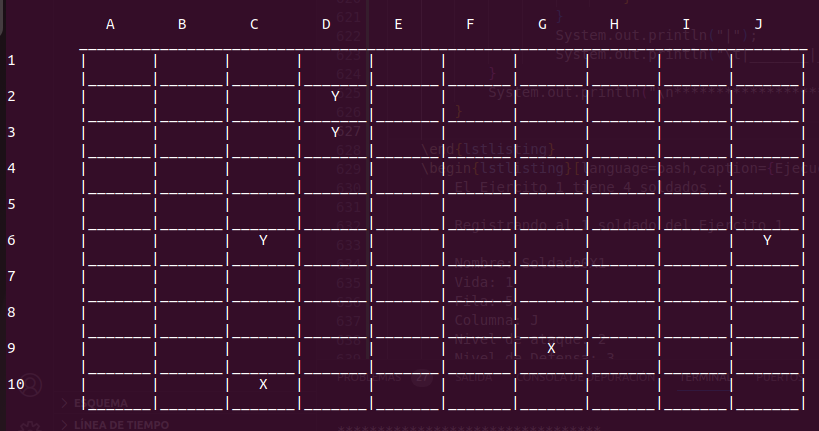
\includegraphics[width=1.0\textwidth,keepaspectratio]{img/Commit3.png}
		%\includesvg{img/automata.svg}
		%\label{img:mot2}
		%\caption{Product backlog.}
	\end{figure}
	\subsection{Ejercicio Soldado}
	\begin{itemize}	
		\item En el cuarto commit creamos el metodo longerLife () tiene la tarea de identificar y mostrar al soldado con la mayor cantidad de vida en un ejercito representado por la matriz bidimensional army. Para ello, inicializa las variables mayor en 0 y soldier como nula, que seran utilizadas para rastrear al soldado con la mayor vida. Luego, mediante bucles anidados, examina todas las casillas de la matriz y compara la vida de cada soldado. Si encuentra un soldado con más vida que el actual registrado en mayor, actualiza esta variable con la vida del soldado y guarda una referencia a ese soldado en soldier. Finalmente, se emite un mensaje que destaca al soldado con la mayor vida en el ejercito correspondiente, identificado por el numero num, y muestra todos los detalles del soldado, como su nombre, salud, posicion y velocidad, permitiendo asi identificar al soldado mas resistente en ese ejercito en particular.
		\item El codigo , el commit y la ejecucion seria el siguiente:
	\end{itemize}	
	\begin{lstlisting}[language=bash,caption={Commit}][H]
		$ git commit -m "El metodo longerLife () tiene la tarea de identificar y mostrar al soldado con la mayor cantidad de vida en un ejercito representado por la matriz bidimensional army. Para ello, inicializa las variables mayor en 0 y soldier como nula, que seran utilizadas para rastrear al soldado con la mayor vida. Luego, mediante bucles anidados, examina todas las casillas de la matriz y compara la vida de cada soldado. Si encuentra un soldado con mas vida que el actual registrado en mayor, actualiza esta variable con la vida del soldado y guarda una referencia a ese soldado en soldier. Finalmente, se emite un mensaje que destaca al soldado con la mayor vida en el ejercito correspondiente, identificado por el numero num, y muestra todos los detalles del soldado, como su nombre, salud, posicion y velocidad, permitiendo asi identificar al soldado mas resistente en ese ejercito en particular."
	\end{lstlisting}	
	\begin{lstlisting}[language=java,caption={Las lineas de codigos del metodo creado:}][H]
		public static void longerLife(ArrayList<ArrayList<Soldado>> army, int num){
			int mayor = 0;//METODO CREADO PARA PODER PERMITIRNOS A CONOCER EL SOLDADO CON MAYOR VIDA DE CADA EJERCITO 
			Soldado soldier = null;
			for(int i = 0; i < army.size(); i++){
				for(int j = 0; j < army.get(i).size(); j++){
					if(army.get(i).get(j) != null){ //COMPROBACION QUE HACEMOS PARA PODER DECIR QUE EL CASILLERO DONDE ESTAMOS ES UN SOLDADO QUE EXISTE
						if(army.get(i).get(j).getLifeActual() > mayor){ //COMPARAMOS PUNTOS DE VIDA DE CADA SOLDADO PARA VER QUIEN ES EL MAYOR 
							mayor = army.get(i).get(j).getLifeActual();
							soldier = army.get(i).get(j);
						}
					}
				}
			}
			System.out.println("El soldado con mayor vida del Ejercito " + num + " es: ");
			System.out.println(soldier.toString());//IMPRIMIMOS SUS DATOS PARA PODER VER DE QUE SOLDADO SE TRATA 
			System.out.println("*********************************");
		}

	\end{lstlisting}
	\begin{lstlisting}[language=bash,caption={Ejecucion:}][H]
		El Ejercito 1 tiene 8 soldados : 

		Registrando al 1 soldado del Ejercito 1
		
		Nombre: Soldado0X1
		Vida: 2
		Fila: 3
		Columna: J
		Nivel de ataque: 1
		Nivel de Defensa: 4
		Nivel de vida: 2
		Velocidad: 5
		Actitud: null
		Estado: true
		---------------------------------
		Registrando al 2 soldado del Ejercito 1
		
		Nombre: Soldado1X1
		Vida: 1
		Fila: 2
		Columna: H
		Nivel de ataque: 2
		Nivel de Defensa: 2
		Nivel de vida: 1
		Velocidad: 1
		Actitud: null
		Estado: true
		---------------------------------
		Registrando al 3 soldado del Ejercito 1
		
		Nombre: Soldado2X1
		Vida: 5
		Fila: 6
		Columna: F
		Nivel de ataque: 3
		Nivel de Defensa: 3
		Nivel de vida: 5
		Velocidad: 2
		Actitud: null
		Estado: true
		---------------------------------
		Registrando al 4 soldado del Ejercito 1
		
		Nombre: Soldado3X1
		Vida: 1
		Fila: 3
		Columna: B
		Nivel de ataque: 3
		Nivel de Defensa: 3
		Nivel de vida: 1
		Velocidad: 5
		Actitud: null
		Estado: true
		---------------------------------
		Registrando al 5 soldado del Ejercito 1
		
		Nombre: Soldado4X1
		Vida: 3
		Fila: 5
		Columna: I
		Nivel de ataque: 2
		Nivel de Defensa: 2
		Nivel de vida: 3
		Velocidad: 2
		Actitud: null
		Estado: true
		---------------------------------
		Registrando al 6 soldado del Ejercito 1
		
		Nombre: Soldado5X1
		Vida: 4
		Fila: 6
		Columna: G
		Nivel de ataque: 3
		Nivel de Defensa: 5
		Nivel de vida: 4
		Velocidad: 4
		Actitud: null
		Estado: true
		---------------------------------
		Registrando al 7 soldado del Ejercito 1
		
		Nombre: Soldado6X1
		Vida: 1
		Fila: 4
		Columna: D
		Nivel de ataque: 4
		Nivel de Defensa: 2
		Nivel de vida: 1
		Velocidad: 4
		Actitud: null
		Estado: true
		---------------------------------
		Registrando al 8 soldado del Ejercito 1
		
		Nombre: Soldado7X1
		Vida: 4
		Fila: 8
		Columna: H
		Nivel de ataque: 4
		Nivel de Defensa: 4
		Nivel de vida: 4
		Velocidad: 5
		Actitud: null
		Estado: true
		---------------------------------
		*********************************
		El Ejercito 2 tiene 10 soldados : 
		
		Registrando al 1 soldado del Ejercito 2
		
		Nombre: Soldado0X2
		Vida: 3
		Fila: 7
		Columna: D
		Nivel de ataque: 1
		Nivel de Defensa: 2
		Nivel de vida: 3
		Velocidad: 1
		Actitud: null
		Estado: true
		---------------------------------
		Registrando al 2 soldado del Ejercito 2
		
		Nombre: Soldado1X2
		Vida: 2
		Fila: 1
		Columna: J
		Nivel de ataque: 3
		Nivel de Defensa: 4
		Nivel de vida: 2
		Velocidad: 5
		Actitud: null
		Estado: true
		---------------------------------
		Registrando al 3 soldado del Ejercito 2
		
		Nombre: Soldado2X2
		Vida: 5
		Fila: 2
		Columna: E
		Nivel de ataque: 4
		Nivel de Defensa: 3
		Nivel de vida: 5
		Velocidad: 3
		Actitud: null
		Estado: true
		---------------------------------
		Registrando al 4 soldado del Ejercito 2
		
		Nombre: Soldado3X2
		Vida: 1
		Fila: 4
		Columna: I
		Nivel de ataque: 5
		Nivel de Defensa: 1
		Nivel de vida: 1
		Velocidad: 1
		Actitud: null
		Estado: true
		---------------------------------
		Registrando al 5 soldado del Ejercito 2
		
		Nombre: Soldado4X2
		Vida: 5
		Fila: 1
		Columna: A
		Nivel de ataque: 2
		Nivel de Defensa: 2
		Nivel de vida: 5
		Velocidad: 5
		Actitud: null
		Estado: true
		---------------------------------
		Registrando al 6 soldado del Ejercito 2
		
		Nombre: Soldado5X2
		Vida: 3
		Fila: 2
		Columna: C
		Nivel de ataque: 1
		Nivel de Defensa: 1
		Nivel de vida: 3
		Velocidad: 3
		Actitud: null
		Estado: true
		---------------------------------
		Registrando al 7 soldado del Ejercito 2
		
		Nombre: Soldado6X2
		Vida: 4
		Fila: 6
		Columna: B
		Nivel de ataque: 4
		Nivel de Defensa: 4
		Nivel de vida: 4
		Velocidad: 2
		Actitud: null
		Estado: true
		---------------------------------
		Registrando al 8 soldado del Ejercito 2
		
		Nombre: Soldado7X2
		Vida: 1
		Fila: 4
		Columna: D
		Nivel de ataque: 5
		Nivel de Defensa: 5
		Nivel de vida: 1
		Velocidad: 4
		Actitud: null
		Estado: true
		---------------------------------
		Registrando al 9 soldado del Ejercito 2
		
		Nombre: Soldado8X2
		Vida: 3
		Fila: 2
		Columna: G
		Nivel de ataque: 4
		Nivel de Defensa: 3
		Nivel de vida: 3
		Velocidad: 3
		Actitud: null
		Estado: true
		---------------------------------
		Registrando al 10 soldado del Ejercito 2
		
		Nombre: Soldado9X2
		Vida: 3
		Fila: 6
		Columna: I
		Nivel de ataque: 4
		Nivel de Defensa: 5
		Nivel de vida: 3
		Velocidad: 1
		Actitud: null
		Estado: true
		---------------------------------
		*********************************
		
		Mostrando tabla de posicion ... --
		Leyenda: Ejercito1 --> X | Ejercito2 --> Y
		
	\end{lstlisting}
	\begin{figure}[H]
		\centering
		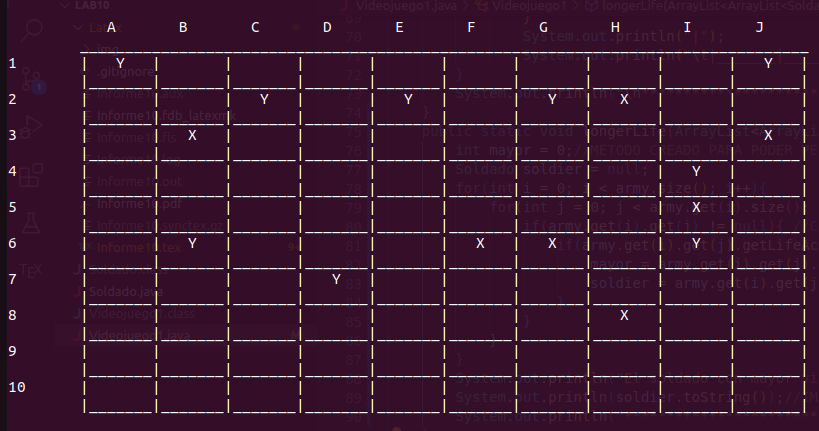
\includegraphics[width=1.0\textwidth,keepaspectratio]{img/Commit4.png}
		%\includesvg{img/automata.svg}
		%\label{img:mot2}
		%\caption{Product backlog.}
	\end{figure}
	\begin{lstlisting}[language=bash,caption={Ejecucion:}][H]
		*********************************
		El soldado con mayor vida del Ejercito 1 es: 
		
		Nombre: Soldado2X1
		Vida: 5
		Fila: 6
		Columna: F
		Nivel de ataque: 3
		Nivel de Defensa: 3
		Nivel de vida: 5
		Velocidad: 2
		Actitud: null
		Estado: true
		*********************************
		El soldado con mayor vida del Ejercito 2 es: 
		
		Nombre: Soldado4X2
		Vida: 5
		Fila: 1
		Columna: A
		Nivel de ataque: 2
		Nivel de Defensa: 2
		Nivel de vida: 5
		Velocidad: 5
		Actitud: null
		Estado: true
		*********************************
		
	\end{lstlisting}
	\subsection{Ejercicio Videojuego1}
	\begin{itemize}	
		\item En el quinto commit creamos el metodo  averageLife() calcula el promedio de los puntos de vida de los soldados en un ejercito representado por una matriz bidimensional llamada army. Comienzo inicializando las variables sum y count en cero. Luego, recorro todas las filas y columnas de la matriz, sumando los puntos de vida de cada soldado a sum y aumentando el contador count. Despues, verifico si el valor de sum es distinto de cero. Si lo es, calculo el promedio dividiendo sum entre count, asegurandome de que el resultado sea un numero decimal, y lo imprimo. Finalmente, devuelvo el valor del promedio. En caso de que sum sea cero (lo que significa que no hay soldados en el ejercito), simplemente imprimo un promedio de vida de 0 y retorno ese valor. Este metodo proporciona el promedio de vida de los soldados en el ejercito identificado por el numero num.
		\item El codigo , el commit y la ejecucion seria el siguiente:
	\end{itemize}	
	\begin{lstlisting}[language=bash,caption={Commit}][H]
		$ git commit -m "Creamos el metodo  averageLife() calcula el promedio de los puntos de vida de los soldados en un ejercito representado por una matriz bidimensional llamada army. Comienzo inicializando las variables sum y count en cero. Luego, recorro todas las filas y columnas de la matriz, sumando los puntos de vida de cada soldado a sum y aumentando el contador count. Despues, verifico si el valor de sum es distinto de cero. Si lo es, calculo el promedio dividiendo sum entre count, asegurandome de que el resultado sea un numero decimal, y lo imprimo. Finalmente, devuelvo el valor del promedio. En caso de que sum sea cero (lo que significa que no hay soldados en el ejercito), simplemente imprimo un promedio de vida de 0 y retorno ese valor. Este metodo proporciona el promedio de vida de los soldados en el ejercito identificado por el numero num"
	\end{lstlisting}	
	\begin{lstlisting}[language=java,caption={Las lineas de codigos del metodo creado:}][H]
		public static double averageLife(ArrayList<ArrayList<Soldado>> army , int num){
			int sum = 0;
			int count = 0;
			System.out.println("El promedio de puntos de vida del Ejercito " + num + " es: ");
			for(int i = 0; i < 10; i++){
				for(int j = 0; j < 10; j++){ //ITERACION LA CUAL NOS AYUDA A PASAR POR TODOS LOS SOLDADOS DE CADA EJERCITO
					if(army.get(i).get(j) != null){ 
						sum += army.get(i).get(j).getLifeActual();
						count++;
					}
				}
			}
			if(sum != 0){
				double avg = sum / (count * 1.0);
				System.out.println(avg); // DAMOS A CONOCER EL PROMEDIO DE VIDA DE CADA EJERCITO 
				System.out.println("*********************************");
				return avg;
			}else{
				double avg = 0;
				System.out.println(avg); // DAMOS A CONOCER EL PROMEDIO DE VIDA DE CADA EJERCITO 
				System.out.println("*********************************");
				return avg;
			}
		}

	\end{lstlisting}
	\begin{lstlisting}[language=bash,caption={Ejecucion:}][H]
		El Ejercito 1 tiene 6 soldados : 

		Registrando al 1 soldado del Ejercito 1
		
		Nombre: Soldado0X1
		Vida: 3
		Fila: 8
		Columna: A
		Nivel de ataque: 3
		Nivel de Defensa: 2
		Nivel de vida: 3
		Velocidad: 4
		Actitud: null
		Estado: true
		---------------------------------
		Registrando al 2 soldado del Ejercito 1
		
		Nombre: Soldado1X1
		Vida: 3
		Fila: 9
		Columna: G
		Nivel de ataque: 5
		Nivel de Defensa: 1
		Nivel de vida: 3
		Velocidad: 3
		Actitud: null
		Estado: true
		---------------------------------
		Registrando al 3 soldado del Ejercito 1
		
		Nombre: Soldado2X1
		Vida: 3
		Fila: 6
		Columna: C
		Nivel de ataque: 5
		Nivel de Defensa: 3
		Nivel de vida: 3
		Velocidad: 2
		Actitud: null
		Estado: true
		---------------------------------
		Registrando al 4 soldado del Ejercito 1
		
		Nombre: Soldado3X1
		Vida: 3
		Fila: 9
		Columna: E
		Nivel de ataque: 5
		Nivel de Defensa: 4
		Nivel de vida: 3
		Velocidad: 4
		Actitud: null
		Estado: true
		---------------------------------
		Registrando al 5 soldado del Ejercito 1
		
		Nombre: Soldado4X1
		Vida: 4
		Fila: 3
		Columna: E
		Nivel de ataque: 3
		Nivel de Defensa: 1
		Nivel de vida: 4
		Velocidad: 5
		Actitud: null
		Estado: true
		---------------------------------
		Registrando al 6 soldado del Ejercito 1
		
		Nombre: Soldado5X1
		Vida: 1
		Fila: 5
		Columna: J
		Nivel de ataque: 1
		Nivel de Defensa: 4
		Nivel de vida: 1
		Velocidad: 4
		Actitud: null
		Estado: true
		---------------------------------
		*********************************
		El Ejercito 2 tiene 8 soldados : 
		
		Registrando al 1 soldado del Ejercito 2
		
		Nombre: Soldado0X2
		Vida: 1
		Fila: 4
		Columna: H
		Nivel de ataque: 2
		Nivel de Defensa: 4
		Nivel de vida: 1
		Velocidad: 3
		Actitud: null
		Estado: true
		---------------------------------
		Registrando al 2 soldado del Ejercito 2
		
		Nombre: Soldado1X2
		Vida: 4
		Fila: 2
		Columna: I
		Nivel de ataque: 4
		Nivel de Defensa: 5
		Nivel de vida: 4
		Velocidad: 5
		Actitud: null
		Estado: true
		---------------------------------
		Registrando al 3 soldado del Ejercito 2
		
		Nombre: Soldado2X2
		Vida: 5
		Fila: 5
		Columna: C
		Nivel de ataque: 4
		Nivel de Defensa: 1
		Nivel de vida: 5
		Velocidad: 1
		Actitud: null
		Estado: true
		---------------------------------
		Registrando al 4 soldado del Ejercito 2
		
		Nombre: Soldado3X2
		Vida: 4
		Fila: 6
		Columna: H
		Nivel de ataque: 1
		Nivel de Defensa: 4
		Nivel de vida: 4
		Velocidad: 1
		Actitud: null
		Estado: true
		---------------------------------
		Registrando al 5 soldado del Ejercito 2
		
		Nombre: Soldado4X2
		Vida: 3
		Fila: 4
		Columna: J
		Nivel de ataque: 3
		Nivel de Defensa: 4
		Nivel de vida: 3
		Velocidad: 3
		Actitud: null
		Estado: true
		---------------------------------
		Registrando al 6 soldado del Ejercito 2
		
		Nombre: Soldado5X2
		Vida: 2
		Fila: 10
		Columna: F
		Nivel de ataque: 2
		Nivel de Defensa: 2
		Nivel de vida: 2
		Velocidad: 5
		Actitud: null
		Estado: true
		---------------------------------
		Registrando al 7 soldado del Ejercito 2
		
		Nombre: Soldado6X2
		Vida: 1
		Fila: 9
		Columna: J
		Nivel de ataque: 4
		Nivel de Defensa: 1
		Nivel de vida: 1
		Velocidad: 1
		Actitud: null
		Estado: true
		---------------------------------
		Registrando al 8 soldado del Ejercito 2
		
		Nombre: Soldado7X2
		Vida: 5
		Fila: 6
		Columna: C
		Nivel de ataque: 2
		Nivel de Defensa: 5
		Nivel de vida: 5
		Velocidad: 4
		Actitud: null
		Estado: true
		---------------------------------
		*********************************
		
		Mostrando tabla de posicion ... --
		Leyenda: Ejercito1 --> X | Ejercito2 --> Y
		
	\end{lstlisting}
	\begin{figure}[H]
		\centering
		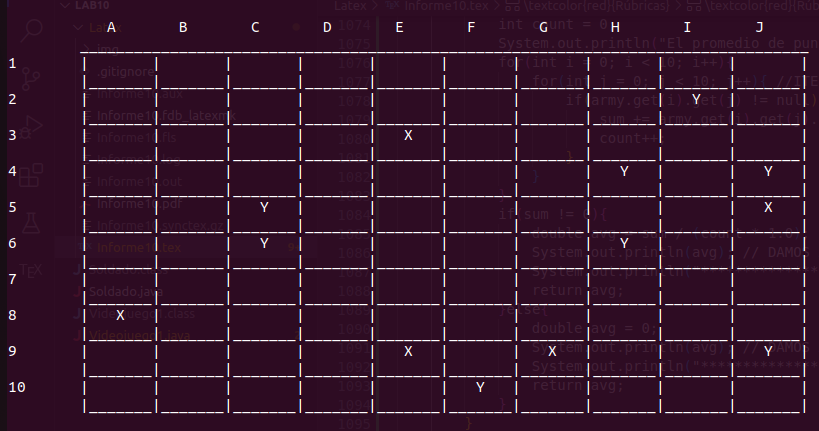
\includegraphics[width=1.0\textwidth,keepaspectratio]{img/Commit5.png}
		%\includesvg{img/automata.svg}
		%\label{img:mot2}
		%\caption{Product backlog.}
	\end{figure}
	\begin{lstlisting}[language=bash,caption={Ejecucion:}][H]
		*********************************
		El soldado con mayor vida del Ejercito 1 es: 
		
		Nombre: Soldado4X1
		Vida: 4
		Fila: 3
		Columna: E
		Nivel de ataque: 3
		Nivel de Defensa: 1
		Nivel de vida: 4
		Velocidad: 5
		Actitud: null
		Estado: true
		*********************************
		El soldado con mayor vida del Ejercito 2 es: 
		
		Nombre: Soldado2X2
		Vida: 5
		Fila: 5
		Columna: C
		Nivel de ataque: 4
		Nivel de Defensa: 1
		Nivel de vida: 5
		Velocidad: 1
		Actitud: null
		Estado: true
		*********************************
		El promedio de puntos de vida del Ejercito 1 es: 
		2.8
		*********************************
		El promedio de puntos de vida del Ejercito 2 es: 
		2.75
		*********************************
		
	\end{lstlisting}
	\subsection{Ejercicio Videojuego1}
	\begin{itemize}	
		\item En el sexto commit creamos el metodo rankingBurbujaLife()  ordena el ranking de soldados en un ejercito representado por la matriz army utilizando el algoritmo de ordenacion burbuja. Primero, cuenta la cantidad de soldados en el ejercito y crea un arreglo llamado soldados para almacenar a estos. Luego, procede a ordenar el arreglo en orden descendente segun la vida de los soldados. Finalmente, muestra el ranking ordenado con los detalles de cada soldado, lo que permite visualizar a los mas saludables en la parte superior del ranking.
		\item El codigo , el commit y la ejecucion seria el siguiente:
	\end{itemize}	
	\begin{lstlisting}[language=bash,caption={Commit}][H]
		$ git commit -m "Creamos el metodo rankingBurbujaLife()  ordena el ranking de soldados en un ejercito representado por la matriz army utilizando el algoritmo de ordenacion burbuja. Primero, cuenta la cantidad de soldados en el ejercito y crea un arreglo llamado soldados para almacenar a estos. Luego, procede a ordenar el arreglo en orden descendente segun la vida de los soldados. Finalmente, muestra el ranking ordenado con los detalles de cada soldado, lo que permite visualizar a los mas saludables en la parte superior del ranking"
	\end{lstlisting}	
	\begin{lstlisting}[language=java,caption={Las lineas de codigos del metodo creado:}][H]
		public static void rankingBurbujaLife(ArrayList<ArrayList<Soldado>> army , int num){
			System.out.println("\nEl Ejercito " + num + " ordenando por metodo burbuja: ");
			int count = 0;
			for(int i = 0; i < 10; i++){
				for(int j = 0; j < 10; j++){ //ITERACION LA CUAL NOS AYUDA A PASAR POR TODOS LOS SOLDADOS DE CADA EJERCITO
					if(army.get(i).get(j) != null){ 
					   count++;
					}
				}
			}
			System.out.println("------------------------------------------");
			System.out.println("Mostrando Ranking del Ejercito " + num + " ..... ////// --->");
			Soldado[] soldados = new Soldado[count];
			int x = 0;
			for(int i = 0; i < 10; i++){
				for(int j = 0; j < 10; j++){ //ITERACION LA CUAL NOS AYUDA A PASAR POR TODOS LOS SOLDADOS AL ARRAY SOLDADO PARA PODER USAR EL USO DEL METODO DE ORDENACION BURBUJA
					if(army.get(i).get(j) != null){ 
						if(count - count + x == count){
							break;
						}else{
							soldados[count - count + x] = army.get(i).get(j);
						}
						x++;   
					}
				}
			}
			int n = soldados.length;
			for (int i = 0; i < n - 1; i++) {
				for (int j = 0; j < n - 1 - i; j++) {
					if (soldados[j].getLifeActual() < soldados[j + 1].getLifeActual()) {
						// Intercambiar elementos si estan en el orden incorrecto
						Soldado temp = soldados[j];
						soldados[j] = soldados[j + 1];
						soldados[j + 1] = temp;
					}
				}
			}
			for(int i = 0; i < soldados.length; i++){
				System.out.print("\n" + "Puesto " + (i + 1));
				System.out.println(soldados[i].toString());
				System.out.println("------------------");
			}
			System.out.println("*********************************");
		}

	\end{lstlisting}
	\begin{lstlisting}[language=bash,caption={Ejecucion:}][H]
		El Ejercito 1 tiene 10 soldados : 

		Registrando al 1 soldado del Ejercito 1
		
		Nombre: Soldado0X1
		Vida: 2
		Fila: 2
		Columna: H
		Nivel de ataque: 2
		Nivel de Defensa: 3
		Nivel de vida: 2
		Velocidad: 4
		Actitud: null
		Estado: true
		---------------------------------
		Registrando al 2 soldado del Ejercito 1
		
		Nombre: Soldado1X1
		Vida: 5
		Fila: 5
		Columna: H
		Nivel de ataque: 3
		Nivel de Defensa: 2
		Nivel de vida: 5
		Velocidad: 2
		Actitud: null
		Estado: true
		---------------------------------
		Registrando al 3 soldado del Ejercito 1
		
		Nombre: Soldado2X1
		Vida: 5
		Fila: 5
		Columna: B
		Nivel de ataque: 5
		Nivel de Defensa: 3
		Nivel de vida: 5
		Velocidad: 5
		Actitud: null
		Estado: true
		---------------------------------
		Registrando al 4 soldado del Ejercito 1
		
		Nombre: Soldado3X1
		Vida: 5
		Fila: 10
		Columna: G
		Nivel de ataque: 1
		Nivel de Defensa: 5
		Nivel de vida: 5
		Velocidad: 4
		Actitud: null
		Estado: true
		---------------------------------
		Registrando al 5 soldado del Ejercito 1
		
		Nombre: Soldado4X1
		Vida: 1
		Fila: 3
		Columna: J
		Nivel de ataque: 4
		Nivel de Defensa: 2
		Nivel de vida: 1
		Velocidad: 1
		Actitud: null
		Estado: true
		---------------------------------
		Registrando al 6 soldado del Ejercito 1
		
		Nombre: Soldado5X1
		Vida: 5
		Fila: 1
		Columna: F
		Nivel de ataque: 3
		Nivel de Defensa: 1
		Nivel de vida: 5
		Velocidad: 3
		Actitud: null
		Estado: true
		---------------------------------
		Registrando al 7 soldado del Ejercito 1
		
		Nombre: Soldado6X1
		Vida: 4
		Fila: 10
		Columna: H
		Nivel de ataque: 3
		Nivel de Defensa: 3
		Nivel de vida: 4
		Velocidad: 4
		Actitud: null
		Estado: true
		---------------------------------
		Registrando al 8 soldado del Ejercito 1
		
		Nombre: Soldado7X1
		Vida: 2
		Fila: 8
		Columna: H
		Nivel de ataque: 3
		Nivel de Defensa: 2
		Nivel de vida: 2
		Velocidad: 1
		Actitud: null
		Estado: true
		---------------------------------
		Registrando al 9 soldado del Ejercito 1
		
		Nombre: Soldado8X1
		Vida: 2
		Fila: 9
		Columna: G
		Nivel de ataque: 3
		Nivel de Defensa: 2
		Nivel de vida: 2
		Velocidad: 4
		Actitud: null
		Estado: true
		---------------------------------
		Registrando al 10 soldado del Ejercito 1
		
		Nombre: Soldado9X1
		Vida: 5
		Fila: 7
		Columna: C
		Nivel de ataque: 5
		Nivel de Defensa: 2
		Nivel de vida: 5
		Velocidad: 2
		Actitud: null
		Estado: true
		---------------------------------
		*********************************
		El Ejercito 2 tiene 6 soldados : 
		
		Registrando al 1 soldado del Ejercito 2
		
		Nombre: Soldado0X2
		Vida: 4
		Fila: 5
		Columna: E
		Nivel de ataque: 1
		Nivel de Defensa: 3
		Nivel de vida: 4
		Velocidad: 2
		Actitud: null
		Estado: true
		---------------------------------
		Registrando al 2 soldado del Ejercito 2
		
		Nombre: Soldado1X2
		Vida: 1
		Fila: 8
		Columna: B
		Nivel de ataque: 4
		Nivel de Defensa: 1
		Nivel de vida: 1
		Velocidad: 3
		Actitud: null
		Estado: true
		---------------------------------
		Registrando al 3 soldado del Ejercito 2
		
		Nombre: Soldado2X2
		Vida: 4
		Fila: 4
		Columna: B
		Nivel de ataque: 1
		Nivel de Defensa: 4
		Nivel de vida: 4
		Velocidad: 5
		Actitud: null
		Estado: true
		---------------------------------
		Registrando al 4 soldado del Ejercito 2
		
		Nombre: Soldado3X2
		Vida: 2
		Fila: 2
		Columna: D
		Nivel de ataque: 1
		Nivel de Defensa: 1
		Nivel de vida: 2
		Velocidad: 5
		Actitud: null
		Estado: true
		---------------------------------
		Registrando al 5 soldado del Ejercito 2
		
		Nombre: Soldado4X2
		Vida: 2
		Fila: 10
		Columna: G
		Nivel de ataque: 3
		Nivel de Defensa: 3
		Nivel de vida: 2
		Velocidad: 5
		Actitud: null
		Estado: true
		---------------------------------
		Registrando al 6 soldado del Ejercito 2
		
		Nombre: Soldado5X2
		Vida: 2
		Fila: 6
		Columna: I
		Nivel de ataque: 1
		Nivel de Defensa: 5
		Nivel de vida: 2
		Velocidad: 2
		Actitud: null
		Estado: true
		---------------------------------
		*********************************
		
		Mostrando tabla de posicion ... --
		Leyenda: Ejercito1 --> X | Ejercito2 --> Y
		
	\end{lstlisting}
	\begin{figure}[H]
		\centering
		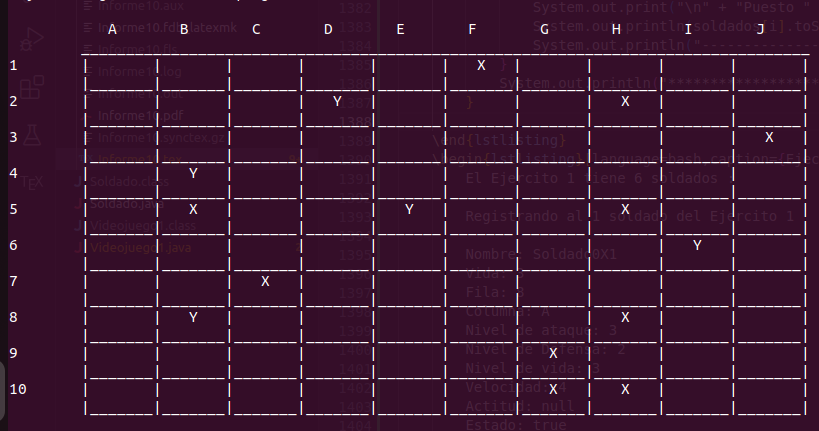
\includegraphics[width=1.0\textwidth,keepaspectratio]{img/Commit6.png}
		%\includesvg{img/automata.svg}
		%\label{img:mot2}
		%\caption{Product backlog.}
	\end{figure}
	\begin{lstlisting}[language=bash,caption={Ejecucion:}][H]
		*********************************
		El soldado con mayor vida del Ejercito 1 es: 
		
		Nombre: Soldado5X1
		Vida: 5
		Fila: 1
		Columna: F
		Nivel de ataque: 3
		Nivel de Defensa: 1
		Nivel de vida: 5
		Velocidad: 3
		Actitud: null
		Estado: true
		*********************************
		El soldado con mayor vida del Ejercito 2 es: 
		
		Nombre: Soldado2X2
		Vida: 4
		Fila: 4
		Columna: B
		Nivel de ataque: 1
		Nivel de Defensa: 4
		Nivel de vida: 4
		Velocidad: 5
		Actitud: null
		Estado: true
		*********************************
		El promedio de puntos de vida del Ejercito 1 es: 
		3.4
		*********************************
		El promedio de puntos de vida del Ejercito 2 es: 
		2.6
		*********************************
		
		El Ejercito 1 ordenando por metodo burbuja: 
		------------------------------------------
		Mostrando Ranking del Ejercito 1 ..... ////// --->
		
		Puesto 1
		Nombre: Soldado5X1
		Vida: 5
		Fila: 1
		Columna: F
		Nivel de ataque: 3
		Nivel de Defensa: 1
		Nivel de vida: 5
		Velocidad: 3
		Actitud: null
		Estado: true
		------------------
		
		Puesto 2
		Nombre: Soldado2X1
		Vida: 5
		Fila: 5
		Columna: B
		Nivel de ataque: 5
		Nivel de Defensa: 3
		Nivel de vida: 5
		Velocidad: 5
		Actitud: null
		Estado: true
		------------------
		
		Puesto 3
		Nombre: Soldado1X1
		Vida: 5
		Fila: 5
		Columna: H
		Nivel de ataque: 3
		Nivel de Defensa: 2
		Nivel de vida: 5
		Velocidad: 2
		Actitud: null
		Estado: true
		------------------
		
		Puesto 4
		Nombre: Soldado9X1
		Vida: 5
		Fila: 7
		Columna: C
		Nivel de ataque: 5
		Nivel de Defensa: 2
		Nivel de vida: 5
		Velocidad: 2
		Actitud: null
		Estado: true
		------------------
		
		Puesto 5
		Nombre: Soldado6X1
		Vida: 4
		Fila: 10
		Columna: H
		Nivel de ataque: 3
		Nivel de Defensa: 3
		Nivel de vida: 4
		Velocidad: 4
		Actitud: null
		Estado: true
		------------------
		
		Puesto 6
		Nombre: Soldado3X1
		Vida: 3
		Fila: 10
		Columna: G
		Nivel de ataque: 1
		Nivel de Defensa: 5
		Nivel de vida: 5
		Velocidad: 4
		Actitud: null
		Estado: true
		------------------
		
		Puesto 7
		Nombre: Soldado0X1
		Vida: 2
		Fila: 2
		Columna: H
		Nivel de ataque: 2
		Nivel de Defensa: 3
		Nivel de vida: 2
		Velocidad: 4
		Actitud: null
		Estado: true
		------------------
		
		Puesto 8
		Nombre: Soldado7X1
		Vida: 2
		Fila: 8
		Columna: H
		Nivel de ataque: 3
		Nivel de Defensa: 2
		Nivel de vida: 2
		Velocidad: 1
		Actitud: null
		Estado: true
		------------------
		
		Puesto 9
		Nombre: Soldado8X1
		Vida: 2
		Fila: 9
		Columna: G
		Nivel de ataque: 3
		Nivel de Defensa: 2
		Nivel de vida: 2
		Velocidad: 4
		Actitud: null
		Estado: true
		------------------
		
		Puesto 10
		Nombre: Soldado4X1
		Vida: 1
		Fila: 3
		Columna: J
		Nivel de ataque: 4
		Nivel de Defensa: 2
		Nivel de vida: 1
		Velocidad: 1
		Actitud: null
		Estado: true
		------------------
		*********************************
		
		El Ejercito 2 ordenando por metodo burbuja: 
		------------------------------------------
		Mostrando Ranking del Ejercito 2 ..... ////// --->
		
		Puesto 1
		Nombre: Soldado2X2
		Vida: 4
		Fila: 4
		Columna: B
		Nivel de ataque: 1
		Nivel de Defensa: 4
		Nivel de vida: 4
		Velocidad: 5
		Actitud: null
		Estado: true
		------------------
		
		Puesto 2
		Nombre: Soldado0X2
		Vida: 4
		Fila: 5
		Columna: E
		Nivel de ataque: 1
		Nivel de Defensa: 3
		Nivel de vida: 4
		Velocidad: 2
		Actitud: null
		Estado: true
		------------------
		
		Puesto 3
		Nombre: Soldado3X2
		Vida: 2
		Fila: 2
		Columna: D
		Nivel de ataque: 1
		Nivel de Defensa: 1
		Nivel de vida: 2
		Velocidad: 5
		Actitud: null
		Estado: true
		------------------
		
		Puesto 4
		Nombre: Soldado5X2
		Vida: 2
		Fila: 6
		Columna: I
		Nivel de ataque: 1
		Nivel de Defensa: 5
		Nivel de vida: 2
		Velocidad: 2
		Actitud: null
		Estado: true
		------------------
		
		Puesto 5
		Nombre: Soldado1X2
		Vida: 1
		Fila: 8
		Columna: B
		Nivel de ataque: 4
		Nivel de Defensa: 1
		Nivel de vida: 1
		Velocidad: 3
		Actitud: null
		Estado: true
		------------------
		*********************************
		
	\end{lstlisting}
	\subsection{Ejercicio Videojuego1}
	\begin{itemize}	
		\item En el septimo commit creamos el metodo rankingInsercionLife() busca ordenar el ranking de los soldados en un ejercito representado por la matriz army mediante el algoritmo de ordenacion por insercion. En primer lugar, se calcula la cantidad de soldados en el ejercito y se crea un arreglo llamado soldados para almacenarlos. Luego, se copian los soldados de la matriz army al arreglo soldados. A continuacion, se procede a ordenar el arreglo soldados en orden descendente segun la vida de los soldados utilizando el algoritmo de ordenacion por insercion. Este proceso implica comparar cada soldado con los que le preceden y reubicarlos en la posicion adecuada. Finalmente, se muestra el ranking ordenado de los soldados, incluyendo su posicion en el ranking y sus detalles, como nombre, salud, posicion y velocidad, lo que permite visualizar a los soldados mas saludables en la parte superior del ranking en funcion de su vida
		\item El codigo , el commit y la ejecucion seria el siguiente:
	\end{itemize}	
	\begin{lstlisting}[language=bash,caption={Commit}][H]
		$ git commit -m "Creamos el metodo rankingInsercionLife() busca ordenar el ranking de los soldados en un ejercito representado por la matriz army mediante el algoritmo de ordenacion por insercion. En primer lugar, se calcula la cantidad de soldados en el ejercito y se crea un arreglo llamado soldados para almacenarlos. Luego, se copian los soldados de la matriz army al arreglo soldados. A continuacion, se procede a ordenar el arreglo soldados en orden descendente segun la vida de los soldados utilizando el algoritmo de ordenacion por insercion. Este proceso implica comparar cada soldado con los que le preceden y reubicarlos en la posicion adecuada. Finalmente, se muestra el ranking ordenado de los soldados, incluyendo su posicion en el ranking y sus detalles, como nombre, salud, posicion y velocidad, lo que permite visualizar a los soldados mas saludables en la parte superior del ranking en funcion de su vida"
	\end{lstlisting}	
	\begin{lstlisting}[language=java,caption={Las lineas de codigos del metodo creado:}][H]
		public static void rankingInsercionLife(ArrayList<ArrayList<Soldado>> army , int num){
			System.out.println("\nEl Ejercito " + num + " ordenando por metodo insercion: ");
			int count = 0;
			for(int i = 0; i < 10; i++){
				for(int j = 0; j < 10; j++){ //ITERACION LA CUAL NOS AYUDA A PASAR POR TODOS LOS SOLDADOS DE CADA EJERCITO
					if(army.get(i).get(j) != null){ 
					   count++;
					}
				}
			}
			System.out.println("------------------------------------------");
			System.out.println("Mostrando Ranking del Ejercito " + num + " ..... ////// --->");
			Soldado[] soldados = new Soldado[count];
			int x = 0;
			for(int i = 0; i < 10; i++){
				for(int j = 0; j < 10; j++){ //ITERACION LA CUAL NOS AYUDA A PASAR POR TODOS LOS SOLDADOS AL ARRAY SOLDADO PARA PODER USAR EL USO DEL METODO DE ORDENACION INSERCION
					if(army.get(i).get(j) != null){ 
						if(count - count + x == count){
							break;
						}else{
							soldados[count - count + x] = army.get(i).get(j); //LA MISMA LOGICA QUE EL ANTERIOR METODO SOLO QUE EN ESTE LO USARIAMOS DE MANERA DIFERENTE YA QUE ESTE SERIA DE FORMA DE INSERCION
						}
						x++;   
					}
				}
			}
			int n = soldados.length;
			for (int i = 1; i < n; i++) {
				Soldado actual = soldados[i];
				int j = i - 1;
				while (j >= 0 && soldados[j].getLifeActual() < actual.getLifeActual()) { //ORDENAMOS EL EJERCITO RESPECTIVAMENTE MEDIANTE EL METODO QUE NOS OFRECE INSERCION EL CUAL ES ESTE CODIGO
					soldados[j + 1] = soldados[j];
					j--;
				}
				soldados[j + 1] = actual;
			}
			for(int i = 0; i < soldados.length; i++){
				System.out.print("\n" + "Puesto " + (i + 1));
				System.out.println(soldados[i].toString()); //PUBLICAMOS RESULTADOS
				System.out.println("------------------");
			}
			System.out.println("*********************************");
		}

	\end{lstlisting}
	\begin{lstlisting}[language=bash,caption={Ejecucion:}][H]
		El Ejercito 1 tiene 1 soldados : 

		Registrando al 1 soldado del Ejercito 1

		Nombre: Soldado0X1
		Vida: 3
		Fila: 3
		Columna: D
		Nivel de ataque: 5
		Nivel de Defensa: 2
		Nivel de vida: 3
		Velocidad: 2
		Actitud: null
		Estado: true
		---------------------------------
		*********************************
		El Ejercito 2 tiene 4 soldados : 

		Registrando al 1 soldado del Ejercito 2

		Nombre: Soldado0X2
		Vida: 4
		Fila: 9
		Columna: F
		Nivel de ataque: 5
		Nivel de Defensa: 1
		Nivel de vida: 4
		Velocidad: 2
		Actitud: null
		Estado: true
		---------------------------------
		Registrando al 2 soldado del Ejercito 2

		Nombre: Soldado1X2
		Vida: 1
		Fila: 5
		Columna: A
		Nivel de ataque: 5
		Nivel de Defensa: 3
		Nivel de vida: 1
		Velocidad: 1
		Actitud: null
		Estado: true
		---------------------------------
		Registrando al 3 soldado del Ejercito 2

		Nombre: Soldado2X2
		Vida: 3
		Fila: 1
		Columna: C
		Nivel de ataque: 1
		Nivel de Defensa: 1
		Nivel de vida: 3
		Velocidad: 5
		Actitud: null
		Estado: true
		---------------------------------
		Registrando al 4 soldado del Ejercito 2

		Nombre: Soldado3X2
		Vida: 3
		Fila: 3
		Columna: I
		Nivel de ataque: 4
		Nivel de Defensa: 3
		Nivel de vida: 3
		Velocidad: 1
		Actitud: null
		Estado: true
		---------------------------------
		*********************************

		Mostrando tabla de posicion ... --
		Leyenda: Ejercito1 --> X | Ejercito2 --> Y

	\end{lstlisting}
	\begin{figure}[H]
		\centering
		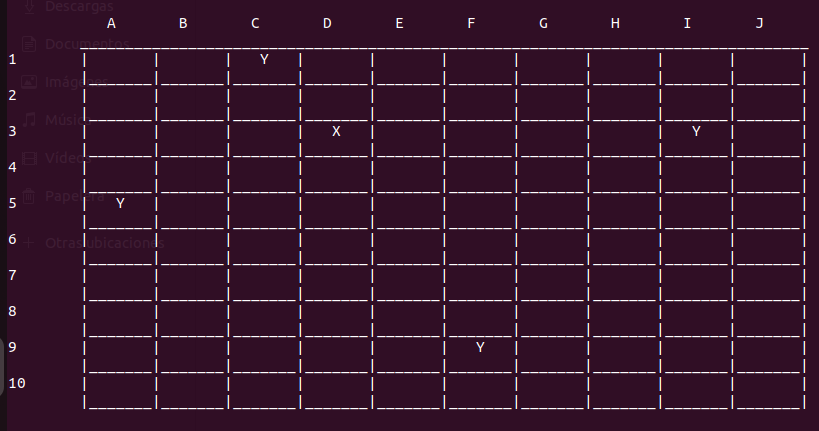
\includegraphics[width=1.0\textwidth,keepaspectratio]{img/Commit7.png}
		%\includesvg{img/automata.svg}
		%\label{img:mot2}
		%\caption{Product backlog.}
	\end{figure}
	\begin{lstlisting}[language=bash,caption={Ejecucion:}][H]
		*********************************
		El soldado con mayor vida del Ejercito 1 es: 
		
		Nombre: Soldado0X1
		Vida: 3
		Fila: 3
		Columna: D
		Nivel de ataque: 5
		Nivel de Defensa: 2
		Nivel de vida: 3
		Velocidad: 2
		Actitud: null
		Estado: true
		*********************************
		El soldado con mayor vida del Ejercito 2 es: 
		
		Nombre: Soldado0X2
		Vida: 4
		Fila: 9
		Columna: F
		Nivel de ataque: 5
		Nivel de Defensa: 1
		Nivel de vida: 4
		Velocidad: 2
		Actitud: null
		Estado: true
		*********************************
		El promedio de puntos de vida del Ejercito 1 es: 
		3.0
		*********************************
		El promedio de puntos de vida del Ejercito 2 es: 
		2.75
		*********************************
		
		El Ejercito 1 ordenando por metodo burbuja: 
		------------------------------------------
		Mostrando Ranking del Ejercito 1 ..... ////// --->
		
		Puesto 1
		Nombre: Soldado0X1
		Vida: 3
		Fila: 3
		Columna: D
		Nivel de ataque: 5
		Nivel de Defensa: 2
		Nivel de vida: 3
		Velocidad: 2
		Actitud: null
		Estado: true
		------------------
		*********************************
		
		El Ejercito 2 ordenando por metodo burbuja: 
		------------------------------------------
		Mostrando Ranking del Ejercito 2 ..... ////// --->
		
		Puesto 1
		Nombre: Soldado0X2
		Vida: 4
		Fila: 9
		Columna: F
		Nivel de ataque: 5
		Nivel de Defensa: 1
		Nivel de vida: 4
		Velocidad: 2
		Actitud: null
		Estado: true
		------------------
		
		Puesto 2
		Nombre: Soldado2X2
		Vida: 3
		Fila: 1
		Columna: C
		Nivel de ataque: 1
		Nivel de Defensa: 1
		Nivel de vida: 3
		Velocidad: 5
		Actitud: null
		Estado: true
		------------------
		
		Puesto 3
		Nombre: Soldado3X2
		Vida: 3
		Fila: 3
		Columna: I
		Nivel de ataque: 4
		Nivel de Defensa: 3
		Nivel de vida: 3
		Velocidad: 1
		Actitud: null
		Estado: true
		------------------
		
		Puesto 4
		Nombre: Soldado1X2
		Vida: 1
		Fila: 5
		Columna: A
		Nivel de ataque: 5
		Nivel de Defensa: 3
		Nivel de vida: 1
		Velocidad: 1
		Actitud: null
		Estado: true
		------------------
		*********************************
		
		El Ejercito 1 ordenando por metodo insercion: 
		------------------------------------------
		Mostrando Ranking del Ejercito 1 ..... ////// --->
		
		Puesto 1
		Nombre: Soldado0X1
		Vida: 3
		Fila: 3
		Columna: D
		Nivel de ataque: 5
		Nivel de Defensa: 2
		Nivel de vida: 3
		Velocidad: 2
		Actitud: null
		Estado: true
		------------------
		*********************************
		
		El Ejercito 2 ordenando por metodo insercion: 
		------------------------------------------
		Mostrando Ranking del Ejercito 2 ..... ////// --->
		
		Puesto 1
		Nombre: Soldado0X2
		Vida: 4
		Fila: 9
		Columna: F
		Nivel de ataque: 5
		Nivel de Defensa: 1
		Nivel de vida: 4
		Velocidad: 2
		Actitud: null
		Estado: true
		------------------
		
		Puesto 2
		Nombre: Soldado2X2
		Vida: 3
		Fila: 1
		Columna: C
		Nivel de ataque: 1
		Nivel de Defensa: 1
		Nivel de vida: 3
		Velocidad: 5
		Actitud: null
		Estado: true
		------------------
		
		Puesto 3
		Nombre: Soldado3X2
		Vida: 3
		Fila: 3
		Columna: I
		Nivel de ataque: 4
		Nivel de Defensa: 3
		Nivel de vida: 3
		Velocidad: 1
		Actitud: null
		Estado: true
		------------------
		
		Puesto 4
		Nombre: Soldado1X2
		Vida: 1
		Fila: 5
		Columna: A
		Nivel de ataque: 5
		Nivel de Defensa: 3
		Nivel de vida: 1
		Velocidad: 1
		Actitud: null
		Estado: true
		------------------
		*********************************
		
	\end{lstlisting}
	\subsection{Estructura de laboratorio 10}
	\begin{itemize}	
		\item El contenido que se entrega en este laboratorio10 es el siguiente:
	\end{itemize}
	\begin{lstlisting}[style=ascii-tree]
	/Lab10	
		"PONER RAMA"

	\end{lstlisting}    
	\section{\textcolor{red}{Rúbricas}}
	
	\subsection{\textcolor{red}{Entregable Informe}}
	\begin{table}[H]
		\caption{Tipo de Informe}
		\setlength{\tabcolsep}{0.5em} % for the horizontal padding
		{\renewcommand{\arraystretch}{1.5}% for the vertical padding
		\begin{tabular}{|p{3cm}|p{12cm}|}
			\hline
			\multicolumn{2}{|c|}{\textbf{\textcolor{red}{Informe}}}  \\
			\hline 
			\textbf{\textcolor{red}{Latex}} & \textcolor{blue}{El informe está en formato PDF desde Latex,  con un formato limpio (buena presentación) y facil de leer.}   \\ 
			\hline 
			
			
		\end{tabular}
	}
	\end{table}
	
	\clearpage
	
	\subsection{\textcolor{red}{Rúbrica para el contenido del Informe y demostración}}
	\begin{itemize}			
		\item El alumno debe marcar o dejar en blanco en celdas de la columna \textbf{Checklist} si cumplio con el ítem correspondiente.
		\item Si un alumno supera la fecha de entrega,  su calificación será sobre la nota mínima aprobada, siempre y cuando cumpla con todos lo items.
		\item El alumno debe autocalificarse en la columna \textbf{Estudiante} de acuerdo a la siguiente tabla:
	
		\begin{table}[ht]
			\caption{Niveles de desempeño}
			\begin{center}
			\begin{tabular}{ccccc}
    			\hline
    			 & \multicolumn{4}{c}{Nivel}\\
    			\cline{1-5}
    			\textbf{Puntos} & Insatisfactorio 25\%& En Proceso 50\% & Satisfactorio 75\% & Sobresaliente 100\%\\
    			\textbf{2.0}&0.5&1.0&1.5&2.0\\
    			\textbf{4.0}&1.0&2.0&3.0&4.0\\
    		\hline
			\end{tabular}
		\end{center}
	\end{table}	
	
	\end{itemize}
	
	\begin{table}[H]
		\caption{Rúbrica para contenido del Informe y demostración}
		\setlength{\tabcolsep}{0.5em} % for the horizontal padding
		{\renewcommand{\arraystretch}{1.5}% for the vertical padding
		%\begin{center}
		\begin{tabular}{|p{2.7cm}|p{7cm}|x{1.3cm}|p{1.2cm}|p{1.5cm}|p{1.1cm}|}
			\hline
    		\multicolumn{2}{|c|}{Contenido y demostración} & Puntos & Checklist & Estudiante & Profesor\\
			\hline
			\textbf{1. GitHub} & Hay enlace URL activo del directorio para el  laboratorio hacia su repositorio GitHub con código fuente terminado y fácil de revisar. &2 &X &2 & \\ 
			\hline
			\textbf{2. Commits} &  Hay capturas de pantalla de los commits más importantes con sus explicaciones detalladas. (El profesor puede preguntar para refrendar calificación). &4 &X &4 & \\ 
			\hline 
			\textbf{3. Código fuente} &  Hay porciones de código fuente importantes con numeración y explicaciones detalladas de sus funciones. &2 &X &2 & \\ 
			\hline 
			\textbf{4. Ejecución} & Se incluyen ejecuciones/pruebas del código fuente  explicadas gradualmente. &2 &X &2 & \\ 
			\hline			
			\textbf{5. Pregunta} & Se responde con completitud a la pregunta formulada en la tarea.  (El profesor puede preguntar para refrendar calificación).  &2 &X &2 & \\ 
			\hline	
			\textbf{6. Fechas} & Las fechas de modificación del código fuente estan dentro de los plazos de fecha de entrega establecidos. &2 &X &2 & \\ 
			\hline 
			\textbf{7. Ortografía} & El documento no muestra errores ortográficos. &2 &X &2 & \\ 
			\hline 
			\textbf{8. Madurez} & El Informe muestra de manera general una evolución de la madurez del código fuente,  explicaciones puntuales pero precisas y un acabado impecable.   (El profesor puede preguntar para refrendar calificación).  &4 &X &2 & \\ 
			\hline
			\multicolumn{2}{|c|}{\textbf{Total}} &20 & &18 & \\ 
			\hline
		\end{tabular}
		%\end{center}
		%\label{tab:multicol}
		}
	\end{table}
	
\clearpage

\section{Referencias}
\begin{itemize}			
	\item \url{https://drive.google.com/drive/u/1/folders/19TzLFO-T77qG7bOWmg5OH7FXAMD2CrJL}
\end{itemize}	
	
%\clearpage
%\bibliographystyle{apalike}
%\bibliographystyle{IEEEtranN}
%\bibliography{bibliography}
			
\end{document}